
\section{Programme scientifique et technique, organisation du projet / Scientific and technical programme, Project organisation}
\begin{xcomment}  
A titre indicatif : de 5 à 10  pages pour ce chapitre, en fonction du nombre de tâches
\end{xcomment}

\subsection{Programme scientifique et structuration du projet  / Scientific programme, project structure}
\begin{xcomment}  
 Pr\'esentez le programme scientifique et justifiez la d\'ecomposition en tâches du programme de travail en coh\'erence avec les objectifs poursuivis. 
Utilisez un diagramme pour pr\'esenter les liens entre les diff\'erentes tâches (organigramme technique)
Les tâches repr\'esentent les grandes phases du projet. Elles sont en nombre limit\'e.
Le cas \'ech\'eant (programmes exigeant la pluridisciplinarit\'e), d\'emontrer l'articulation entre les disciplines scientifiques.
N'oubliez pas les tâches correspondant à la diss\'emination et à la valorisation, à d\'ecrire en d\'etails au §4.

\end{xcomment}

The DADA project includes fundamental research in multiple disciplines, focusing on a single object of study - the virtual actor. Work will be divided into four main work packages: (1) procedural animation of isolated actors; (2) procedural animation of interaction between actors; (3) authoring and real-time control; (4) user evaluations. 

\begin{figure}[htbp]
\begin{center}
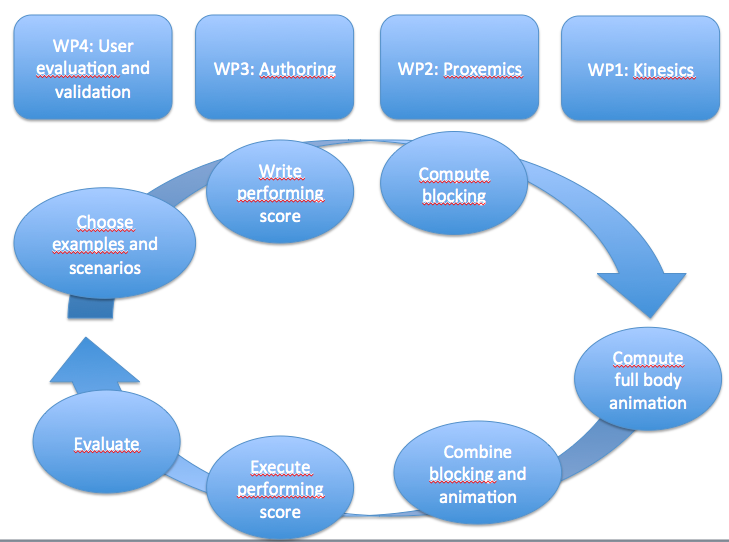
\includegraphics[width=\linewidth]{DADAWORKFLOW.png}
\caption{Data flow between work packages: Through the authoring tool (WP3), a script is elaborated by a theater director (WP4); it gives direction to group of actors which act out autonomously the commands of the script to position toward each other and in the virtual space (WP2). The behaviors of each actor is computed taking into account their emotional states and social relations (WP1).}
\label{default}
\end{center}
\end{figure}



\begin{xcomment}  
thierry : ce passage là doit probablement etre remonté au dessus pour l'explication générale du flux entre WPs. 
\end{xcomment}


WP4 focuses on ...

WP3 focuses on ...

WP2 focuses on ...


WP1 focuses on animation models for isolated actors.  The inputs that are used by the methods to be developped in this WP are procedural animation scenario as output by WP2.  Such a scenario includes in particular detailed indications on the action to be realized (walk from one point to another, carry object, knock on door, throw object, lift object, move object), the mood of the character (neutral, happy, afraid, angry, anxious, sad, proud, shameful) and a set of static information about the character that change the way people move (age, gender, morphology, corpulence, expressivity level, etc). Both action and mood may vary with time among the animation while static information remain fixed per nature.  These three sets of information will be refered hereafter as \textit{action context}, \textit{mood context} and \textit{profile context}. . 


\endinput